\section{System Overview}
\label{overview}
\noindent
Heimdall has two components: the first is an app installed on a user's mobile device and the second is a Web service that receives install, uninstall and update notifications when these events occur on the device. Upon notification, the server processes all heuristics that apply to the app and generates a set of actions for a system administrator. At this point the system generates a list of recommended actions and sends it over to the Heimdall Mobile App. Our present prototype, includes sample content provider heuristics. The server also allows a system administrator to add more heuristics and add action notifications to be sent to a mobile device in a BYOD scenario.

\begin{figure}[tb]
	\centering
	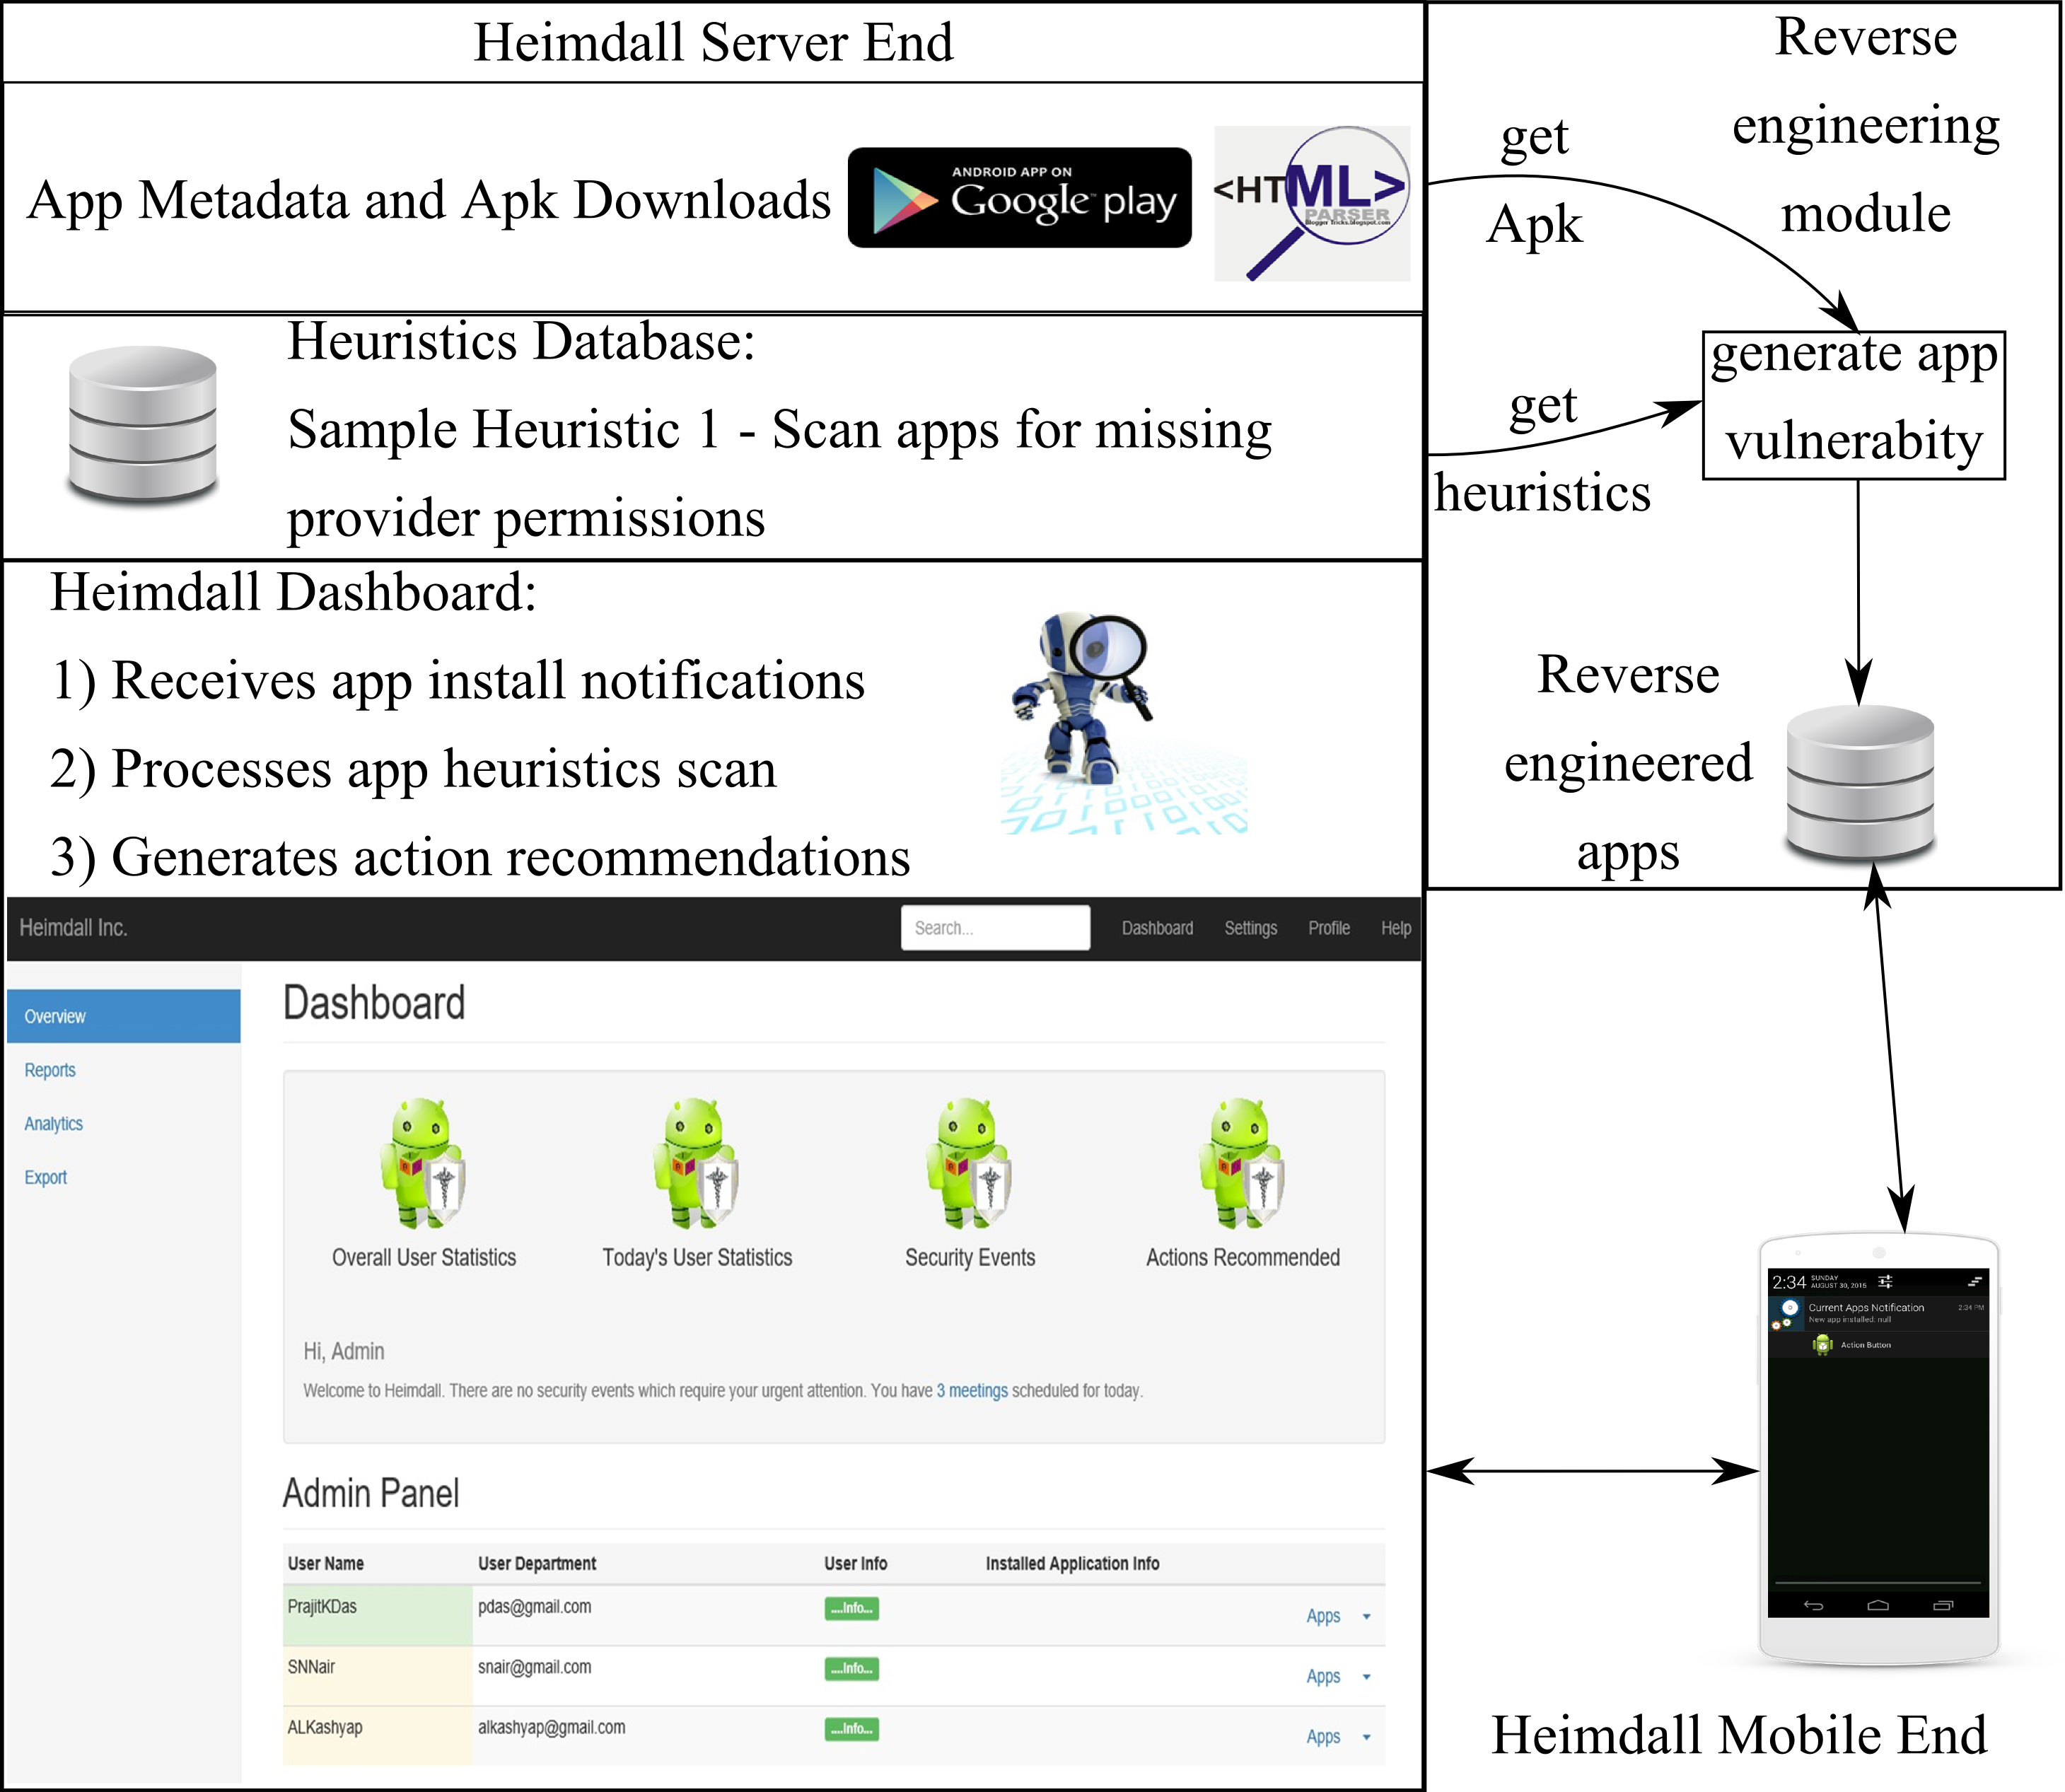
\includegraphics[width=\columnwidth]{images/architecture}
	\caption{System Overview}
	\label{fig:arch}
\end{figure}

Heimdall server has two capabilities. Heimdall can generate reverse engineered apps that we then test on the mobile devices. The reverse engineering process takes into account the heuristics that allow us to detect vulnerability apps and introduces them into the apps we repackage. For example we discuss a vulnerability in the next section where content providers on android could have a potential breach of data. We introduce this vulnerability into any provider associated with the apps we are reverse engineering and we remove associated permissions and ensure that the ``exported'' tag for the provider is set to true. Naturally the primary task of Heimdall is to detect the vulnerabilities in the apps. Vulnerabilities that might include missing provider permissions for apps. For demonstrating these capabilities, we downloaded about 1500 apps from the Google Play Store. We used a tool called apktool~\footnote{A tool for reverse engineering 3rd party, closed, binary Android apps~\url{https://ibotpeaches.github.io/Apktool/}} to decompile the Android binary application packages (apks) and parse the manifest files to find providers and thus determine whether the apps are vulnerable or not. At the same time if they are not already vulnerable we can introduce the vulnerability and repackage the app for testing purposes. We are working on including more heuristics into Heimdall to make it capable of detecting many more vulnerabilities.